%\documentclass{beamer}
\documentclass[brown]{beamer}
\usepackage{beamerthemesplit}
%\usepackage{beamerthemeshadow}
%\usetheme{default} 

\usepackage{amsfonts}
\usepackage{amssymb}
\usepackage{amsmath}
\usepackage{dsfont}
\usepackage{graphicx}
\usepackage{varioref}

\usepackage{color}
\definecolor{yellow}{rgb}{1,1,0}
\definecolor{black}{rgb}{0,0,0}
\definecolor{ltcyan}{rgb}{.75,1,1}
\definecolor{blue}{rgb}{0,0,1}
\definecolor{red}{rgb}{1,0,0}
\definecolor{darkred}{rgb}{0.5,0,0}
\definecolor{darkgreen}{rgb}{0,0.5,0}

\usepackage{listings}
\lstloadlanguages{C,C++}
\lstset{fontadjust=false,basicstyle=\small\ttfamily}
\lstset{language=C}
\lstdefinelanguage{Dax}{
  morekeywords={WorkMapField,WorkMapCell,Cell,Field,FieldCell,FieldPoint,FieldCoordinates,Scalar,Vector3,Vector4},
  morekeywords={[2]dax,exec,comp,void},
  morekeywords={[3]DAX_WORKLET,DAX_IN,DAX_OUT}
}
\lstset{
  keywordstyle=\color{blue},
  keywordstyle=[2]\color{darkred},
  keywordstyle=[3]\color{darkgreen}
}

\newcommand*{\textC}[1]{\texttt{#1}}
\newcommand\mysection[1]{
  \section{#1}
  \begin{frame}
    \begin{center}{\LARGE
      #1
      }
    \end{center}
  \end{frame}
}

% removes the mark from footnote.
\let\thefootnote\relax\footnotetext{Footnotetext without footnote mark} 

\title{\textbf{Dax Toolkit}: \\
  A Proposed Framework for Data Analysis \\
  and Visualization at Extreme Scale\footnote
    {
  This work was supported in full by the DOE Office of Science, Advanced
  Scientific Computing Research, under award number 10-014707, program manager
  Lucy Nowell.
    }
}

\author{\small
  Kenneth Moreland {\tiny Sandia National Laboratories} \\
  \textbf{Utkarsh Ayachit} {\tiny Kitware, Inc. } \\
  Berk Geveci {\tiny Kitware, Inc. }\\
  Kwan-Liu Ma {\tiny University of California at Davis}
}
%\author{Kenneth Moreland \\
%\textbf{Utkarsh Ayachit} \\
%Berk Geveci\\
%Kwan-Liu Ma}
\date {October 24, 2011}

\setbeamertemplate{footline}{}
\beamertemplatenavigationsymbolsempty

\begin{document}
\frame{\titlepage}

%\section{Introduction}
\frame
{
  %\frametitle{In this talk...}
  \begin{beamerboxesrounded}{Dax Toolkit}
  A new visualization framework designed to exhibit the pervasive parallelism
    necessary for exascale machines.
  \end{beamerboxesrounded}
}

\mysection{Motivation}
\subsection{Background}

\frame
{
  \frametitle{Visualization Pipeline}
  % Talk about the visualization pipeline.
  \begin{figure}
  \centering
  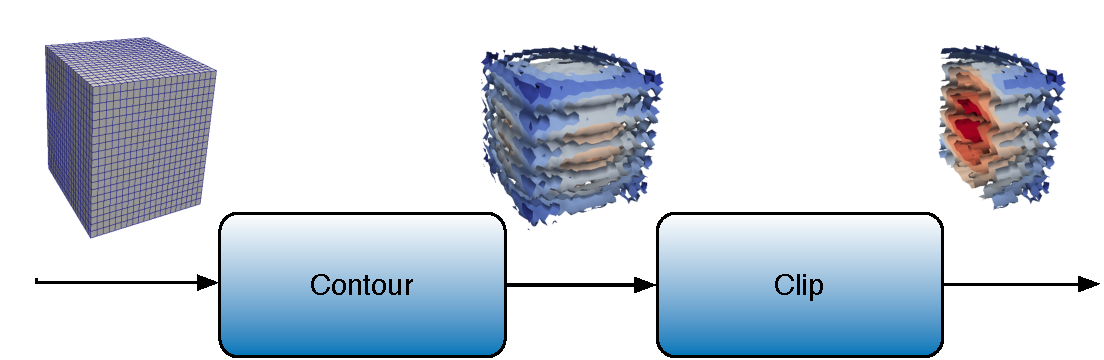
\includegraphics[width=.8\textwidth]{images/SimplePipeline.pdf}
  \end{figure}
}

\frame
{
  \frametitle{Parallel Visualization Pipeline}
  %Talk about how VTK/ParaView/VisIt deal with parallelism.
  \begin{figure}
  \centering
  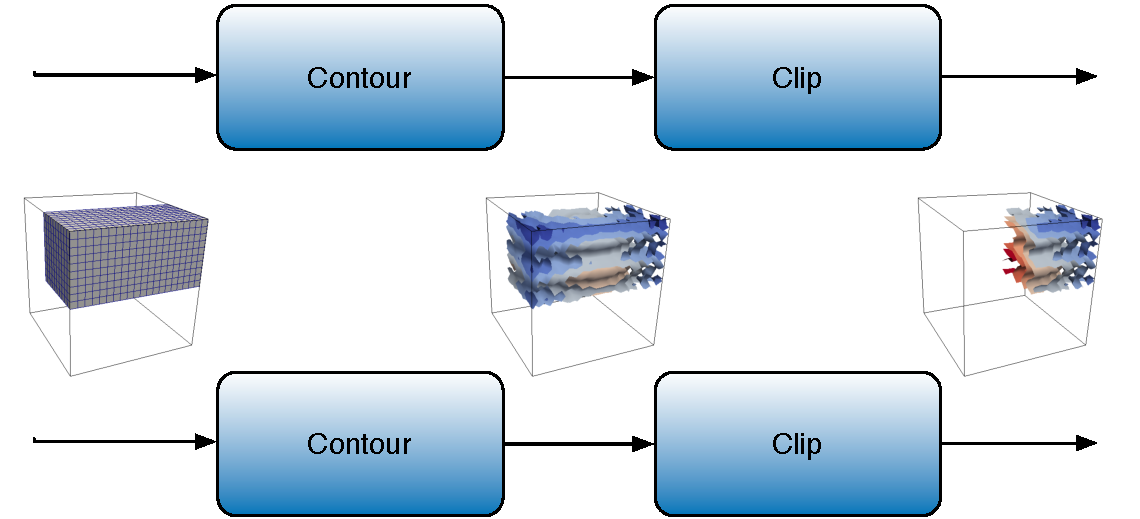
\includegraphics[width=.8\textwidth]{images/ParallelVisPipeline.pdf}
  \end{figure}
}


\frame
{
  \frametitle{Petascale To Exascale\footnote[1]{Estimates consolidated from International
  Exascale Software Project Roadmap and the DOE Exascale Initiative Roadmap.}}
  \renewcommand{\arraystretch}{1.5}
  \begin{table}[htbp]
    \centering
    \begin{tabular}{l|l|l|l}
      & Jaguar -- XT5 & Exascale & Increase \\
      \hline
      Cores & 224,256
      & 100 million -- 1 billion
      & 400 -- 5,000$\times$ \\
      Threads & 224,256 way
      & 1 -- 10 billion way
      & 4,000 -- 50,000$\times$ \\
      Memory & 300 Terabytes
      & 10 -- 128  Petabytes
      & 30 -- 500$\times$
    \end{tabular}
  \end{table}
}

\subsection{Our Approach}
\frame
{
  \frametitle{Revisiting the Filter}
  \begin{figure}
  \centering
  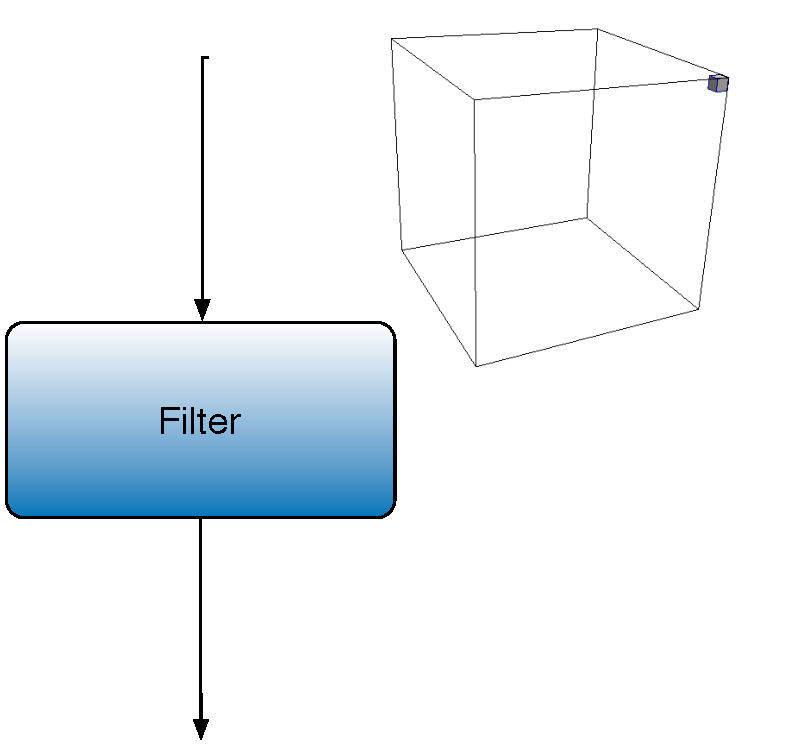
\includegraphics[width=0.5\textwidth]{images/SingleElementFilter.pdf}
  \end{figure}
}

\frame
{
  \begin{center}
  {\ttfamily
  function (\emph{in}, \emph{out})}
  \end{center}
}

\frame
{
  \begin{center}
  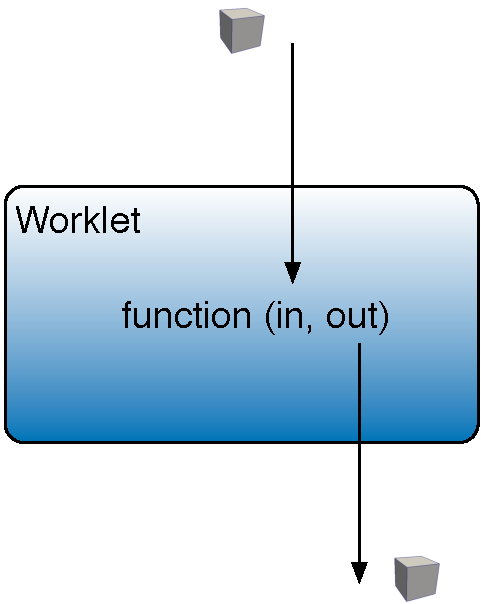
\includegraphics[width=0.3\textwidth]{images/worklet.pdf}
  \end{center}
}

\frame
{
  \begin{center}
  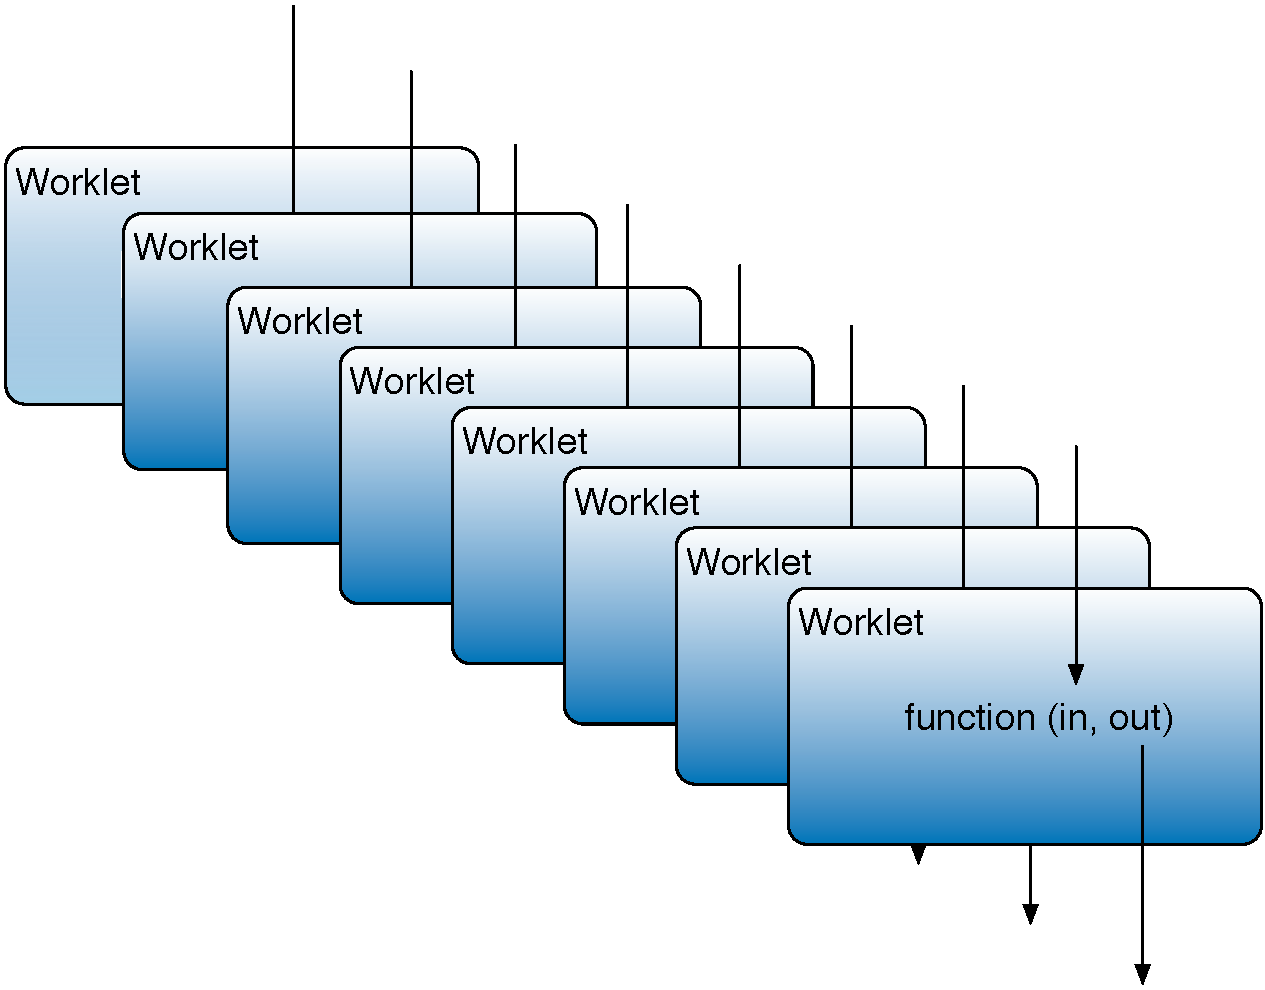
\includegraphics[width=\textwidth]{images/many_worklets.pdf}
  \end{center}
}

\subsection{Related Work}
\frame
{
  \frametitle{Existing Approaches}
  Multicore extensions to VTK pipeline [Vo, et al. 2010]
  % The stuff that Huy from Utah did with multicore.
  \begin{itemize}
  \item Pros: Can be applied to most existing VTK filters.
  \item Cons: High overhead for each execution thread; VTK algorithms
    optimized for sizeable chunks.
  \end{itemize}
  Functional field definitions (FEL/FM) [Bryson, et al. 1996]
  % Fields are defined as functions, kind of like a the basic field map in
  % Dax.  Berk knows more about it than I do.
  \begin{itemize}
  \item Pros: Mesh flexibility; low memory overhead; lazy evaluation;
    straighforward to parallelize.
  \item Cons: Does not manage massive multi-threading; no mechanism for
    topology generation.
  \end{itemize}
  MapReduce [Dean and Ghemawat 2008] [Vo, et al. 2011]
  % MapReduce is a database technology designed to do custom query like
  % operations on large, irregular, sparse data sets.  To program in
  % MapReduce, you provide to functions: a map and a reduce.  The map
  % function is applied to every record in the database.  Looking at the
  % one record, it produces key/value pairs.  The system collects the
  % key/value pairs and groups all such pairs with the same key in a global
  % shuffling operation.  Each group with the same key is then given to the
  % reduce function, which produces output for that group.  Before you in
  % the same session as your talk Huy should be presenting this.
  %
  % The first con is that the abstractions provided by MapReduce are
  % principally for database queries.  It is difficult to cast
  % visualization algorithms in the system.  It also throws away some
  % a priori knowledge about the mesh.  The shuffling operation is global
  % when in general it does not have to be.  Key matches could be
  % restricted to known neighbors or within domain decompositions, but
  % MapReduce does not know about that.
  \begin{itemize}
  \item Pros: simple programming model for massive parallelism; custom
    systems specializing in large amounts of data.
  \item Cons: Difficult to cast visualization algorithms; global shuffling
    opeartion inefficient because it ignores known neighborhood or domain
    decompositions.
  \end{itemize}
}

\mysection{Dax Toolkit}
\subsection{Overview}

\frame
{
  \frametitle{Implementation Assumptions}
  \begin{itemize}
  \item GPU $\approx$ Exascale Node
  \item CUDA $\approx$ Development Environment on Exascale Node
  \end{itemize}
}

\frame
{
  \frametitle{Dax Programming Environment}
  \begin{figure}[htbp]
    \centering
    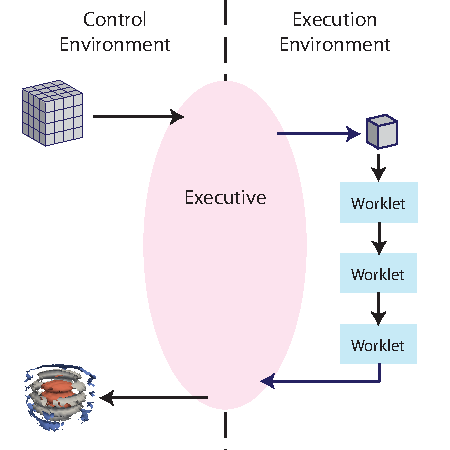
\includegraphics[width=.6\textwidth]{images/DaxDiagram}
  \end{figure}
}

\begin{frame}[fragile]
\frametitle{Data Model}

\begin{itemize}
\item %
\begin{lstlisting}[language=Dax]
dax::exec::Work
\end{lstlisting} %

Corresponds to \emph{work} performed by each Worklet. %
\begin{lstlisting}[language=Dax]
dax::exec::WorkMapField
dax::exec::WorkMapCell
\end{lstlisting}

\item %
\begin{lstlisting}[language=Dax]
dax::exec::Field
\end{lstlisting}%

Provides access to data arrays. %
\begin{lstlisting}[language=Dax]
dax::exec::Field
dax::exec::FieldCell
dax::exec::FieldPoint
dax::exec::FieldCoordinates
\end{lstlisting}
\end{itemize}
\end{frame}


\subsection{Execution Environment}
\begin{frame}[fragile]
\frametitle{Execution Environment}
\begin{lstlisting}[language=Dax]
DAX_WORKLET void FieldWorklet(
    DAX_IN dax::exec::WorkMapField& work,
    DAX_IN dax::exec::Field& in_field,
    DAX_OUT dax::exec::Field& out_field)
{
  dax::Scalar in_value = in_field.GetScalar(work);
  dax::Scalar out_value = ...;
  out_field.Set(work, out_value);
}
\end{lstlisting}
\end{frame}

\subsection{Control Environment}
\frame
{
  \frametitle{Control Environment}
  Example of how the control environment looks.
}

\mysection{Results}

\begin{frame}[fragile]
\frametitle{Code Comparison}
\begin{columns}[l]
\column{.49\linewidth}
\begin{lstlisting}[language=C++,basicstyle=\tiny\ttfamily]
int vtkCellDerivatives::RequestData(...)
{
  ...[allocate output arrays]...
  ...[validate inputs]...
  for (cellId=0; cellId < numCells; cellId++)
    {
    ...[update progress]...
    input->GetCell(cellId, cell);
    subId = cell->GetParametricCenter(
                              pcoords);
    inScalars->GetTuples(
      cell->PointIds, cellScalars);
    scalars = cellScalars->GetPointer(0);
    cell->Derivatives(
     subId,
     pcoords,
     scalars,
     1,
     derivs);
    outGradients->SetTuple(cellId, derivs);
    }
  ...[cleanup]...
}
\end{lstlisting}

\column{.49\linewidth}
\begin{lstlisting}[language=Dax, basicstyle=\tiny\ttfamily]
DAX_WORKLET void CellGradient(...)
{





  dax::exec::Cell cell(work);
  dax::Vector3 parametric_cell_center
    = dax::make_Vector3(0.5, 0.5, 0.5);
 

  dax::Vector3 value = cell.Derivative(
    parametric_cell_center,
    points,
    point_attribute,
    0);


  cell_attribute.Set(work, value);


}
\end{lstlisting}
\end{columns}
\end{frame}

\frame
{
  \frametitle{Performance Comparison}
  \begin{table}[htbp]
    \centering
    \label{tab:Results}
    %\vspace{6pt}
    \begin{tabular}{llrrr}
      \qquad & Mesh Size & VTK Time & Dax Time & Speedup \\
      \hline
      \multicolumn{5}{l}{Elevation $\rightarrow$ Gradient} \\
      %% & $144^3$ & 2.75 s & 0.02 (0.03) s & 138 (92) \\
      %% & $256^3$ &  15.52 s & 0.11 (0.19) s & 141 (82) \\
      %% & $512^3$ &  125.75 s & 0.89 (1.57) s &  141 (80) \\
      & $144^3$ & 2.75 s & 0.013 (0.024) s & 210 (114) \\
      & $256^3$ &  15.52 s & 0.074 (0.135) s & 210 (115) \\
      & $512^3$ &  125.75 s & 0.589 (1.076) s &  213 (117) \\
      \multicolumn{5}{l}{Elevation $\rightarrow$ Sine $\rightarrow$ Square $\rightarrow$ Cosine} \\
      & $144^3$ & 2.32 s & 0.002 (0.006) s &  1169 (386) \\
      & $256^3$ &  12.99 s & 0.013 (0.034) s & 999 (382) \\
      & $512^3$ & 103.88 s & 0.110 (0.276) s &  944 (376) \\
    \end{tabular} 
  \end{table}
  {Performance comparison between Dax toolkit and VTK. Values in
  parentheses show the corresponding values with data transfer times
  included}.
}

\frame
{
  \frametitle{Ongoing Work}
  Summarize the challenges ahead and some of the ongoing work.
}

\frame
{
  \frametitle{Conclusion}
  Dax Toolkit
}

\frame
{
  \frametitle{Acknowledgements}
  This work was supported in full by the DOE Office of Science, Advanced
  Scientific Computing Research, under award number 10-014707, program manager
  Lucy Nowell.
}

\end{document}
